\newpage
\section{Active Composite State}

\subsection{Mathematical Representation}

\noindent As \textit{Active} is a composite state, it is defined as the tuple $S = (Q, \Sigma_1, \Sigma_2, q_0, V, \Lambda)$, where\\

\noindent $Q = \{Start~Setting, Setting, Setting~Complete, Washing, Rinse, Spin\}$\\
\noindent $\Sigma_1 = \{cancel, press~button~for~cycle~type, program~set, washing~complete, after(3 mins), after(2 mins)\}$\\
\noindent $\Sigma_2 = \{reset~settings, lock~door, unlock~door\}$\\
\noindent $q_0: Start~Setting$\\
\noindent $V: door = \{open, closed\}$\\
\noindent $\Lambda$: Transition specifications\\
\indent 1. $\rightarrow \textit{Start Setting}$\\
\indent 2. $\textit{Start Setting} \rightarrow Setting$\\
\indent 3. $Setting \xrightarrow {\text {cancel/reset settings}} \textit{Start Setting}$\\
\indent 4. $Setting \xrightarrow {\text {press button for cycle type}} \textit{Setting Complete}$\\
\indent 5. $\textit{Setting Complete} \xrightarrow {\text {program set [door is closed] / lock door}} Washing$\\
\indent 6. $Washing \xrightarrow {\text {washing complete}} Rinse$\\
\indent 7. $Rinse \xrightarrow {\text {after(3min)}} Spin$\\
\indent 8. $Spin \xrightarrow {\text {after(2min) / unlock door}} Exit$\\

\noindent The UML state diagram is shown in Figure~\ref{fig:Active}.

\newpage
\subsection{State transition diagram}

\begin{figure}[h!]
	\centering
		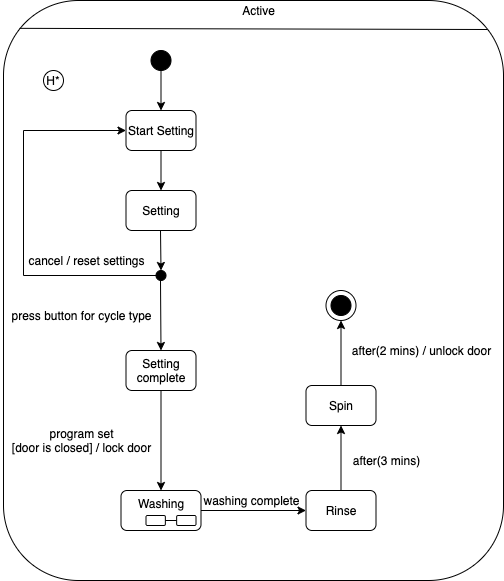
\includegraphics[width=0.8\textwidth]{Active}
		  \caption{Active State Diagram}\label{fig:Active}
\end{figure}
